\documentclass[11pt]{article}
\usepackage{ctable,microtype,natbib,amsmath,amssymb,fullpage,graphicx}
\usepackage{siunitx}
\usepackage{cleveref}
\usepackage{keyval,kvoptions,fancyvrb,float,ifthen,calc,ifplatform,pdftexcmds,etoolbox,lineno}
\usepackage[utf8]{inputenc}
\usepackage{color}
\usepackage[danish]{babel}
\usepackage[left=25mm, right=25mm, top=25mm, bottom=25mm]{geometry}
\usepackage{lastpage}
\usepackage{amsthm}
\setlength\parindent{0pt}
\usepackage{fancyhdr}
\usepackage{dcolumn}
\usepackage{minted} 
\usepackage{setspace}

\onehalfspacing

\title{Hardware}
\author{Christian Bondesen - 201511621}

\begin{document}
\maketitle
\section{Implementering og test: }
I implementerings- og testdelen af hardwaren tjekkes der om de forskellige hardware-dele, gør det som er forventet. Her testes de 4 forskellige dele, X-10 modtager, X-10 sender og 2 gange Zero-cross. Der vil først ske en implementering af Zero-cross og X-10 sender, herefter vil de testes for at se om det gør som forventet. Herefter vil der ske en implemtering af X-10 modtager der efterfulgt vil blive testet sammen med Zero-cross. Herunder ses et billede af helesystemet samlet:
\begin{figure}[H]
\centering
\includegraphics[scale = 0.08]{HeleSystemHardware}
\caption{Billede af hele systemet implementeret samlet}
\end{figure}
\subsection{Zero-cross og X-10 sender}
Dette afsnit gennemgås implementeringen af Zero-cross og X-10 sender. Hvorefter der efterfulgt vil gennemgås en test af begge implementeringer. \subsubsection{Zero-cross:}
\label{sec:Zero-cross}
Herunder ses en implementering af Zero-cross.
\begin{figure}[H]
\centering
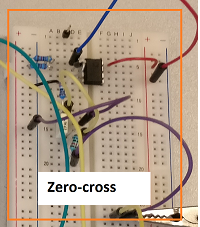
\includegraphics[scale = 1.5]{Zerocrossimplementering}
\caption{Zero-cross implementering}
\end{figure}
Implementering af Zero-cross er lavet som beskrevet i designfasen. For at teste om Zero-crossingen gør som der er forventet, er der lavet et program som detekterer hvert zero cross. Da Zero-cross hardwaren blev testet blev der erfaret at der for hver nulgennemgang. (billede?). Der er 2 Zero-cross, en på X-10 modtager og X-10 sender. De har samme funktion derfor er det nok bare at teste den ene. Herunder ses et billede af testen: 
\begin{figure}[H]
\centering
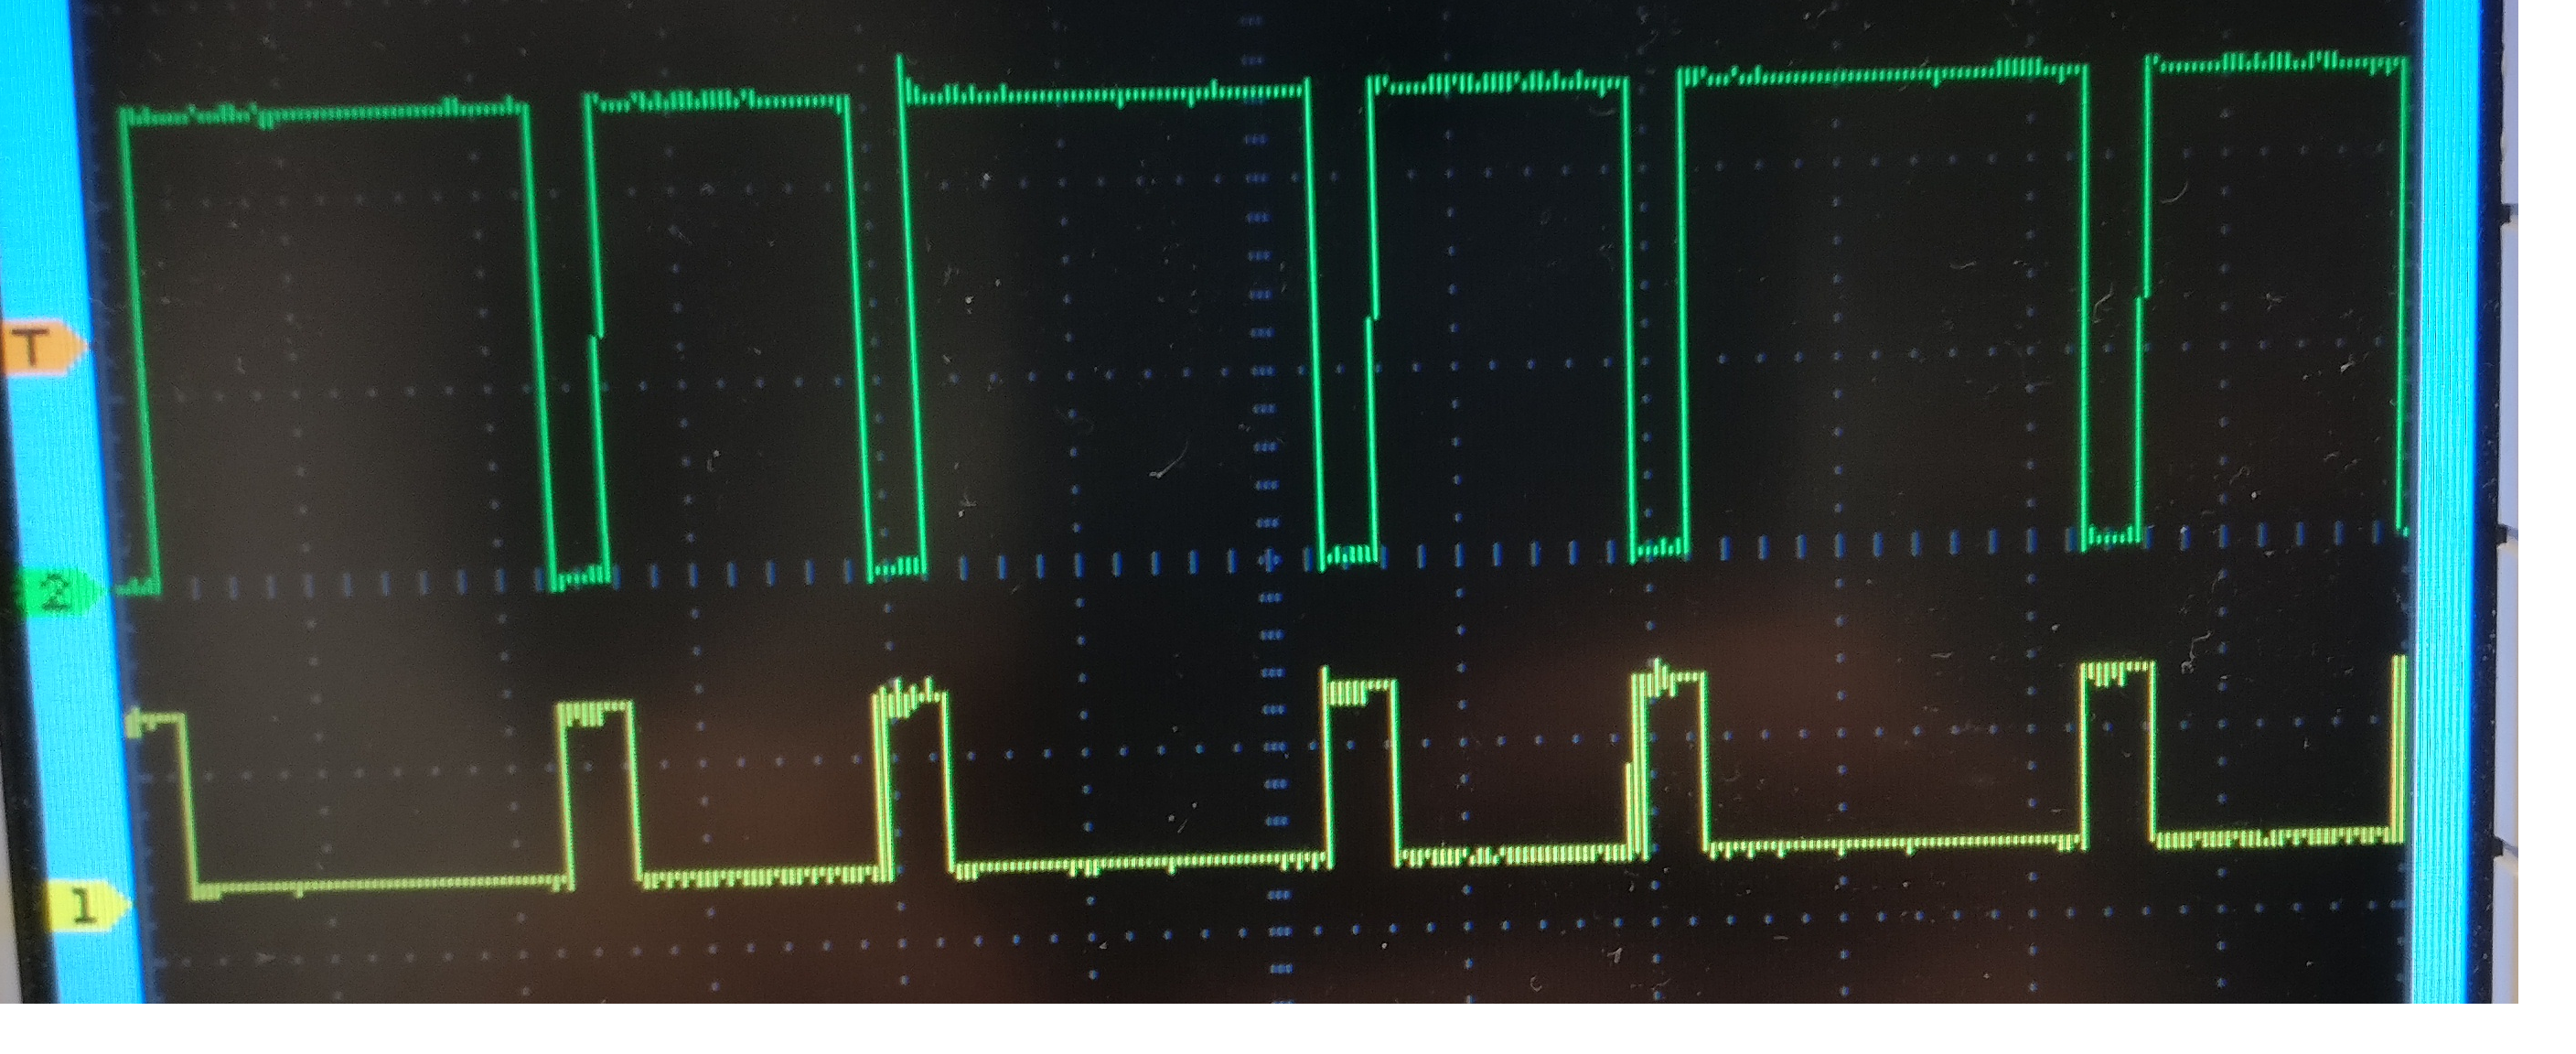
\includegraphics[scale = 0.2]{zerocrosstest}
\caption{Zero-cross test med implementering udfra desgin}
\end{figure}
Den grønne lysnettes 18 VAC efter Op-amp'en, den gule er Zero-cross detekteret på ATmega2560. I næste section vil X-10 sender gennengås.
\subsubsection{X-10 sender:}
Herunder ses implementeringen af X-10 sender.
\begin{figure}[H]
\centering
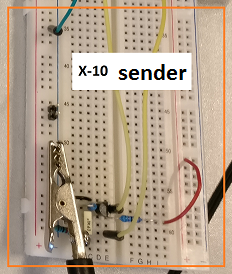
\includegraphics[scale = 1]{X-10sender}
\caption{Billede af implementering af X-10 sender}
\end{figure}
For at teste X-10 senderen bliver der simuleret et burst signal med Analog-Discovery. Der kan tændes og slukkes for burst'ne. Herunder ses et billede at testen for X-10 senderen. Der er valgt at sende burst på \SI{120}{\kilo\hertz} for hvert \SI{8.3}{\micro\second}.
\begin{figure}[H]
\centering
\includegraphics[scale = 0.1]{Lysnet-sender}
\caption{Billede af lysnettet efter generatoren}
\end{figure}
Lysnettet har nu de burst som der skal detekteres at modtageren. Disse burst skal forestille sig at være et logisk 1-tal når den opfanges af X-10 modtageren. Det ses på figur 5 at X-10 senderen, overlejrer lysnettets AC-signal med et \SI{120}{\kilo\hertz}.
\subsubsection{X-10 sender og Zero-cross}
Der vil nu ske en implemenering og test af Zero-cross og X-10 sender samlet. For at teste dette er der lavet et program på ATmega2560, der for hvert zero-cross sender et \SI{120}{\kilo\hertz} burst. Disse burst går så gennem X-10 sender og derved sender burstne sikkert ud på lysnettet. Herunder ses implementering af X-10 sender og Zero-cross samlet:
\begin{figure}[H]
	\centering
	\includegraphics[scale = 0.2]{implementering-zerocross-sender}
	\caption{Billede af X-10 sender og Zero-cross samlet implementeret}
	\label{fig:SamletImpZXSender}
\end{figure}
Efter implementeringen af Zero-cross og X-10 sender, er der foretaget en test som beskrevet oven for. Der er målt med et osciloskop. Målingerne for testen ses herunder:
\begin{figure}[H]
	\centering
	\includegraphics[scale = 0.1]{osciloskop-af-implementering}
	\caption{Billede af osciloskop-målinger for implementering}
	\label{fig:OscImplementering}
\end{figure}
På billedet kan man se det gule signal som svarer til udgangen på Zero-cross og den grønne som tilsvarer udgangen på X-10 sender. Læg mærke til at der her ikke er noget lysnet sat til vores X-10 sender og derfor kun viser at den overlejrer signalet for hvert Zero-cross. Heraf kan det altså konkluderes at det vil være muligt at sende en bitstreng der kan sendes sikkert over lysnettet.
\subsection{Implementering af X-10 modtager og Zero-cross}
Denne section gennemgås en implementering af X-10 modtager og Zero-cross. Herefter vil der ske en test af begge implementeringer. Da Zero-cross har samme funktion for denne hardware del, vil der ikke ske en fuld gennemgang. Hvis man ønsker at se hele implementering med test refereres der til sektion \ref{sec:Zero-cross} Zero-cross.
\subsubsection{X-10 modtager}
Herunder ses implementeringen af X-10 modtager. Implementeringen er bygget op som vist i designfasen(mangler reference):
\begin{figure}[H]
	\centering
	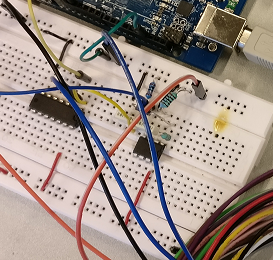
\includegraphics[scale = 1]{X-10modtager-imp}	
	\caption{Billede af implementering for X-10 modtager}
	\label{fig:impX10mod}
\end{figure}
For implementeringen er der brugt osciloskoper for at teste modtageren. Testen foregår ved at der sendes et \SI{120}{\kilo\hertz} signal ud på modtageren vha. Analog Discovery. Herefter kan vi måle med et osciloskop om den skaber et digitalt signal, hvergang den modtager et burst. Dette signal skal senere bruges til ATmega2560, der vil oversætte signalet. Herunder ses et billede af osciloskop målingerne:
\begin{figure}[H]
	\centering
	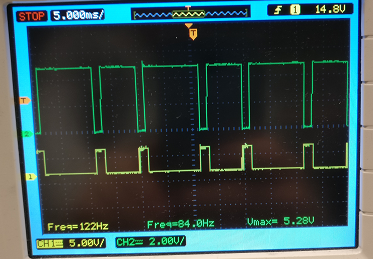
\includegraphics[scale = 1]{X-10modtager-osc}		
	\caption{Billede af osciloskop målingerne for X-10 modtager}
	\label{bil:oscmodtager}
\end{figure}
I testen af X-10 modtager implementeringen ses der som forventet at for hvert burst(gult-signal), vil modtagere detektere et nul(grønt-signal). Den falder fordi at der er en inverterende schmidt-trigger efter envelopen på selve X-10 modtager-delen. Som forventet ses der er at X-10 modtageren kan sortere det høje frekvenssignal fra og skabe et enkelt højt signal på \SI{1}{\milli\second} som kan detekteres af ATmega2560. I næste sektion vil der gennemgås en implemenetering af X-10 modtager sammen med Zero-cross.
\subsubsection{Implementering Zero-cross og X-10 modtager}
Denne sektion gennemgår implementeringen af X-10 modtager og Zero-cross samlet. Herunder ses et billede af implementeringen:
\begin{figure}[H]
	\centering
	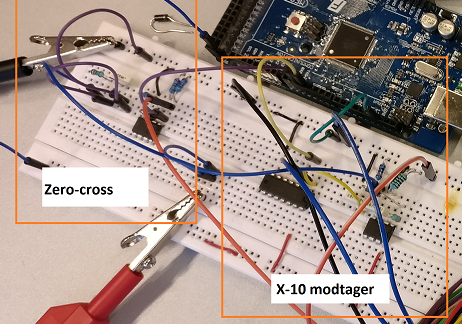
\includegraphics[scale = 0.8]{zeroXmodtagerimp}
	\caption{billede af Zero-cross og X-10 modtager implementering}
	\label{bil:ZeroXmodimp}
\end{figure}
Efterfølgende billede viser en test af de to hardwaredele sammen. Der er testet i håb om at der for hver nulgennemgang vil aflæse en et højt eller et lavt signal. Herunder ses et billede af osciloskop målingerne:
\begin{figure}[H]
	\centering
	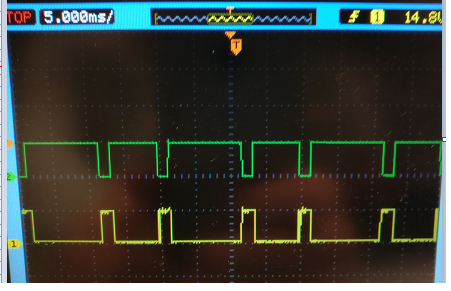
\includegraphics[scale = 1]{zeromodtest}
	\caption{Billede af Zero-cross og X-10 modtager test}
	\label{bil:ZeroXmodtest}
\end{figure}
I testen af X-10 modtager og Zero-cross implementeringen ses der som forventet at for hvert Zero-cross(gult-signal). Vil modtageren læse et højt eller lavt. I dette tilfælde vil den kun læse højesignaler fordi testen er levet med et program der sender et burst for hvert zero-cross. I den næste sektion vil der testes hele systemet samlet. Der er lavet et software test program til ATmega2560 der sender 3 høje signaler og 1 lavt. Implementering og testen ses i næste sektion.


\subsection{Implementering af alle hardware dele}
I denne sektion sker en implementering og en test af de fårige sektioner og hardwaredele, bare samlet. Dvs. der implementeres en fungerende X-10 modtager med Zero-cross sammen med X-10 sender med Zero-cross. Yderligere vil der ske en test af denne implementering. Her forventes det at der sendes et signal på 4 bit, 3 høje og 1 lavt ud på lysnettet. Dette signal vil kunne aflæses med X-10 modtagere delen hvorefter det kan ses på osciloskopet at der kommer samme digitale signal ud. Implementering for hardware delen af hele systemet ses herunder:
\begin{figure}[H]
	\centering
	\includegraphics[scale = 1]{}
	\caption{Caption here}
	\label{fig:figure1}
\end{figure}

\end{document}
